\subsubsection{Sensitivity of the baseline feature scores to the activation threshold}
\label{subsubsection:rebuttal_threshold_sensitivity}

For CEBRA-Time and LangevinFlow, a latent counts as active when its (sign-oriented) value lies in the highest $r$ fraction of eligible development windows, with $r$ set per feature from the reference NLDisco latent ($r=31.921\%$, $0.793\%$, $1.473\%$ and $2.401\%$; \autoref{subsubsection:churchland_results_additional}). To test how much the thresholded scores depend on this choice, we keep every latent shown in \autoref{table:churchland_feature_metrics} fixed (same coordinate and sign) and re-score it on the development windows while the activation rate varies from $0.1\%$ to $60\%$ (\autoref{figure:rebuttal_threshold_sensitivity}). We treat NLDisco in the same way: its latent is thresholded at the corresponding quantile of its activation amplitude, up to the rate at which the threshold reaches its native rule $z>0$ (rates above this are not reachable for a sparse latent because it has no further nonzero activations). We also report each latent's own best threshold, defined as the threshold that maximizes \metric{Sel} on the development windows among thresholds that meet the eligibility rule used for latent selection (\metric{Cov}$\,\geq0.05$ and activity in at least 20 positive trials), for all methods. \metric{AUROC} is computed from the raw activations and does not depend on the threshold (\autoref{table:rebuttal_threshold_sensitivity}). The scores at the paper's rate are recomputed from the saved representations and agree with the scores stored with the selections.

\begin{figure}[!htbp]
    \centering
    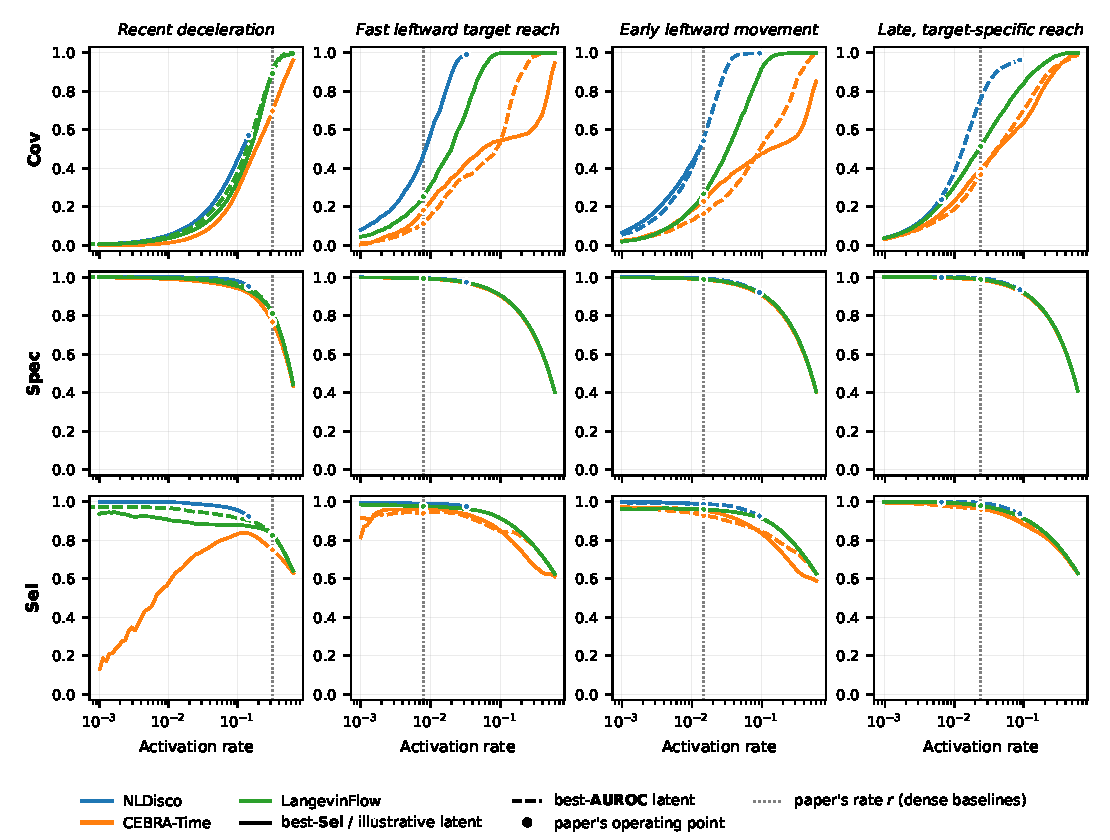
\includegraphics[width=\linewidth]{figures/rebuttal/change09_thresholds/threshold_sensitivity.pdf}
    \caption{\textbf{Threshold sensitivity of \metric{Cov}, \metric{Spec} and \metric{Sel}.} Each column is one behavioral description and each curve one latent from \autoref{table:churchland_feature_metrics}, re-scored on the development windows as the activation rate that sets its threshold varies. Dots mark the paper's operating point (rate $r$ for the dense baselines, dotted vertical line; native threshold $z>0$ for NLDisco, whose curve ends there). Solid lines: best-\metric{Sel} latent (illustrative latent for NLDisco on the two main-text features); dashed lines: best-\metric{AUROC} latent where different.}
    \label{figure:rebuttal_threshold_sensitivity}
\end{figure}

\metric{Cov} rises and \metric{Spec} falls as the rate increases for every method. For the three rarer features, doubling the rate from $r/2$ to $2r$ changes the baseline latents' \metric{Sel} by at most $0.044$, while their \metric{Cov} grows by a factor of $2.0$--$4.2$; for recent deceleration, where $r=31.9\%$ and $2r$ is $63.8\%$, \metric{Sel} falls by $0.20$--$0.26$. \metric{Sel} rises as the threshold tightens and \metric{Cov} falls: at their own best thresholds the baseline latents reach \metric{Sel} of $0.84$--$0.97$ (recent deceleration), $0.95$--$0.98$ (fast leftward target reach), $0.96$--$0.97$ (early leftward movement) and $0.99$--$1.00$ (late, target-specific reach) with \metric{Cov} between $0.05$ and $0.36$. NLDisco's latents reach \metric{Sel} of $0.996$--$1.000$ at their own best thresholds ($\metric{Cov}=0.05$--$0.26$).

At equal coverage, the NLDisco latent has higher \metric{Sel} than the baselines. When each baseline threshold is chosen to maximize \metric{Sel} subject to $\metric{Cov}$ at least that of the reference NLDisco latent, the best baseline \metric{Sel} is $0.899$ for recent deceleration, $0.929$ for fast leftward target reach, $0.808$ for early leftward movement and $0.817$ for late, target-specific reach, compared with $0.924$, $0.975$, $0.926$ and $0.937$ for the NLDisco latent at its native threshold (\autoref{table:churchland_feature_metrics}).

\begin{table}[!htbp]
    \centering
    {\scriptsize\setlength{\tabcolsep}{2.5pt}\renewcommand{\arraystretch}{1.08}
    \resizebox{\linewidth}{!}{\begin{tabular}{llrrrrrrrrrrrrrr}
\toprule
Latent & Selector & \metric{AUROC} & \multicolumn{3}{c}{$r/2$} & \multicolumn{3}{c}{Paper $r$} & \multicolumn{3}{c}{$2r$} & \multicolumn{3}{c}{Own best} & Rate \\
\cmidrule(lr){4-6}\cmidrule(lr){7-9}\cmidrule(lr){10-12}\cmidrule(lr){13-15}
 & & & \metric{Cov} & \metric{Spec} & \metric{Sel} & \metric{Cov} & \metric{Spec} & \metric{Sel} & \metric{Cov} & \metric{Spec} & \metric{Sel} & \metric{Cov} & \metric{Spec} & \metric{Sel} & at best \\
\midrule
\multicolumn{15}{l}{\textit{Recent deceleration}; $r=31.92\%$} \\
NLDisco 83 & illustrative & 0.769 & 0.342 & 0.990 & 0.970 & 0.571 & 0.953 & 0.924 & -- & -- & -- & 0.053 & 1.000 & 0.998 & 0.99\% \\
CEBRA-Time 126 & best Sel/AUROC & 0.818 & 0.452 & 0.907 & 0.830 & 0.698 & 0.767 & 0.750 & 0.961 & 0.436 & 0.630 & 0.359 & 0.932 & 0.840 & 12.24\% \\
LangevinFlow 136 & best Sel & 0.909 & 0.520 & 0.923 & 0.871 & 0.909 & 0.816 & 0.831 & 0.995 & 0.443 & 0.641 & 0.051 & 0.994 & 0.901 & 1.40\% \\
LangevinFlow 178 & best AUROC & 0.922 & 0.575 & 0.935 & 0.899 & 0.892 & 0.812 & 0.826 & 0.998 & 0.444 & 0.642 & 0.051 & 0.998 & 0.967 & 1.09\% \\
\midrule
\multicolumn{15}{l}{\textit{Fast leftward target reach}; $r=0.79\%$} \\
NLDisco 20 & illustrative & 0.990 & 0.794 & 0.990 & 0.987 & 0.991 & 0.975 & 0.975 & -- & -- & -- & 0.052 & 1.000 & 0.996 & 0.06\% \\
CEBRA-Time 93 & best Sel & 0.785 & 0.081 & 0.997 & 0.960 & 0.183 & 0.993 & 0.965 & 0.304 & 0.986 & 0.957 & 0.195 & 0.993 & 0.966 & 0.82\% \\
CEBRA-Time 56 & best AUROC & 0.909 & 0.059 & 0.996 & 0.944 & 0.112 & 0.993 & 0.941 & 0.245 & 0.986 & 0.946 & 0.068 & 0.996 & 0.947 & 0.43\% \\
LangevinFlow 179 & best Sel/AUROC & 0.979 & 0.144 & 0.997 & 0.981 & 0.252 & 0.994 & 0.977 & 0.439 & 0.987 & 0.972 & 0.073 & 0.999 & 0.984 & 0.18\% \\
\midrule
\multicolumn{15}{l}{\textit{Early leftward movement}; $r=1.47\%$} \\
NLDisco 122 & best Sel & 0.768 & 0.348 & 0.998 & 0.993 & 0.542 & 0.993 & 0.987 & -- & -- & -- & 0.065 & 1.000 & 1.000 & 0.10\% \\
NLDisco 40 & best AUROC & 0.991 & 0.991 & 0.968 & 0.968 & 0.998 & 0.921 & 0.926 & -- & -- & -- & 0.055 & 1.000 & 0.996 & 0.10\% \\
CEBRA-Time 93 & best Sel & 0.738 & 0.145 & 0.995 & 0.965 & 0.229 & 0.988 & 0.952 & 0.335 & 0.975 & 0.931 & 0.058 & 0.998 & 0.970 & 0.26\% \\
CEBRA-Time 54 & best AUROC & 0.855 & 0.108 & 0.994 & 0.948 & 0.164 & 0.987 & 0.929 & 0.248 & 0.974 & 0.904 & 0.050 & 0.998 & 0.963 & 0.26\% \\
LangevinFlow 179 & best Sel/AUROC & 0.963 & 0.141 & 0.995 & 0.963 & 0.267 & 0.989 & 0.960 & 0.463 & 0.977 & 0.952 & 0.097 & 0.997 & 0.967 & 0.47\% \\
\midrule
\multicolumn{15}{l}{\textit{Late, target-specific reach}; $r=2.40\%$} \\
NLDisco 165 & best Sel & 0.618 & 0.125 & 1.000 & 1.000 & 0.237 & 1.000 & 0.998 & -- & -- & -- & 0.185 & 1.000 & 1.000 & 0.48\% \\
NLDisco 75 & best AUROC & 0.976 & 0.911 & 0.979 & 0.978 & 0.962 & 0.935 & 0.937 & -- & -- & -- & 0.264 & 1.000 & 1.000 & 0.69\% \\
CEBRA-Time 142 & best Sel & 0.910 & 0.264 & 0.995 & 0.980 & 0.394 & 0.986 & 0.965 & 0.520 & 0.965 & 0.936 & 0.051 & 1.000 & 0.995 & 0.16\% \\
CEBRA-Time 44 & best AUROC & 0.920 & 0.216 & 0.993 & 0.971 & 0.368 & 0.985 & 0.961 & 0.535 & 0.965 & 0.939 & 0.051 & 1.000 & 0.994 & 0.16\% \\
LangevinFlow 136 & best Sel/AUROC & 0.961 & 0.348 & 0.997 & 0.991 & 0.515 & 0.989 & 0.979 & 0.685 & 0.969 & 0.957 & 0.051 & 1.000 & 0.999 & 0.14\% \\
\bottomrule
\end{tabular}
}}
    \caption{\textbf{Scores at named activation-rate settings.} Development windows; latents as in \autoref{table:churchland_feature_metrics}. For the dense baselines, $r/2$, $r$ and $2r$ are multiples of the paper's rate; for NLDisco, $r$ is the native threshold $z>0$, half of its native rate is shown, and twice that rate is not reachable (--). Own best: the threshold with the highest \metric{Sel} subject to $\metric{Cov}\geq0.05$ and activity in at least 20 positive trials; the last column gives the resulting activation rate. \metric{AUROC} does not depend on the threshold.}
    \label{table:rebuttal_threshold_sensitivity}
\end{table}
